%%This is a very basic article template.
%%There is just one section and two subsections.
\documentclass{article}

\usepackage{graphicx}

\begin{document}

\section{Continious Delivery mit Puppet alt. Konfigurationsmangement mit Puppet}

Eine Vielzahl an Applikationen, jede enwickelt mit Agile Methoden von mehreren Teams.

Gebaut wird stündlich oder öfters mit Continous Integration - in unserem Fall \cite{jenkins}.

Die Applikationen sollen automatisch mit verschiedenen Konfigurationen installiert werden und danach - ebenso automatisch - getestet werden.

Da die Applikationen in unterschiedliche Länder eingesetz werden und für jedes
Locale getestet werden sollte, multiplizieren sich die Servers.

Nach hoffentlich erfolgreiche Integrationstests sollten die Applikationen auf
weitere Servers in QA- und Produktionsstufe installiert und konfiguriert.

Zur guter Letz werden die Applikationen im Clusters eingesetzt.

Für die Installation und Konfiguration wird je Applikation Scripts entwickelt. Fallweise mit Copy/Paste verfahren und divergierende Weiterentwicklung.

Dass war die Ausgangssituation als wir angefangen haben uns mit dem Thema Konfigurationsmanagement auseinander zu setzen. Wir haben uns für 
\cite{puppet} entschieden, eine andere Möglichkeit wäre \cite{chef}.

\subsection{Ziele}

More plain text.

\subsection{Entwicklungsumgebung}

Für die Entwicklung von Puppet Module und Manifeste (mehr dazu gleich) kann \cite{geppeto} installiert werden.

Puppet kann unter für Unix mit einem Paketmanager installiert werden oder für Windows von \cite{puppetlabs} runtergeladen werden.

Für die Test von Puppet Module und Manifeste wird hier \cite{vagrant} verwendet. Vagrant setzt auf \cite{openbox} auf. 
Wie Puppet können beide mit dem Paketmanager unter Unix installiert werden oder von der Downloadseite runtergeladen werden.

\subsection{Demo: Apache und eine Webseite mit Puppet installieren}

\subsubsection{Testbox mit Vagrant}
Nachdem Vagrant und VirtualBox installiert worden sind, können wir einen Box zum testen aufsetzen.
Hier wird Debian Squeeze 64 verwendet. Eine Liste mit Vagrant Boxes gibt es auf http://www.vagrantbox.es/

\begin{verbatim}
vagrant box add debian_squeeze_64 http://dl.dropbox.com/u/937870/VMs/squeeze64.box
\end{verbatim}

Die Vagrant Boxen werden unter Unix in \verb \$HOME/.vagrant.d/boxes\end installiert.
Falls man dies ändern will kann man die Umgebungsvariabel \verb VAGRANT_HOME setzen:


\begin{verbatim}
export VAGRANT_HOME=\$HOME/vagrant_home
\end{verbatim}


Nachdem der Vagrant Box \verb debian_squeeze_64 jetzt zur Verfügung steht, können wir den jetzt initialisieren.
\begin{verbatim}
vagrant init debian_squeeze_64
\end{verbatim}

Jetzt können wir den Box starten:
\begin{verbatim}
vagrant up
\end{verbatim}


\begin{figure}[h]
\includegraphics{user.pp.eps}
\caption{User mit Puppet anlegen}
\label{user.pp}
\end{figure}

\author{Michael Haslgrübler}

\author{Anders Malmborg}

\subsection{Referenzen}

\begin{thebibliography}{10}

\bibitem[Jenkins]{jenkins}
	Jenkins: An extendable open source continuous integration server.
  	http://jenkins-ci.org/

\bibitem[Puppet]{puppet}
  	Puppet is IT automation software that helps system administrators manage infrastructure throughout its lifecycle, 
  from provisioning and configuration to patch management and compliance.
  	http://puppetlabs.com/puppet/what-is-puppet/
  
\bibitem[Chef]{chef}
 	Chef is a systems integration framework, built to bring the benefits of configuration management to your entire infrastructure.
  	http://wiki.opscode.com/display/chef/Home

\bibitem[Geppeto Eclipse Plugin]{geppeto}
	Eclipse Plugin for developing Puppet modules and manifests
	https://github.com/cloudsmith/geppetto/wiki

\bibitem[Puppet Labs Downloads]{puppetlabs}
	http://info.puppetlabs.com/download-puppet-open-source.html

\bibitem[Vagrant]{vagrant}
	http://vagrantup.com/
	
\bibitem[VirtualBox]{virtualbox}
	https://www.virtualbox.org/	
		  
\end{thebibliography}

\end{document}
